\documentclass[grado3]{LEMA-Tikz-IM}

\usepackage{graphicx}  % Needed to include graphics
% \usepackage{pifont} % For the scissors symbol

\begin{document}

\newcommand{\setPage}{
  \def\myMargin{1in}
  \def\topMargin{0.7in}
 
  % page canvas letter size
  \path (0,0) rectangle (8.5in,11in);

  \coordinate (botLeft) at (\myMargin,\myMargin);
  \coordinate (botRight) at (8.5in-\myMargin,\myMargin);
  \coordinate (topRight) at (8.5in-\myMargin,11in-\topMargin);
  \coordinate (topLeft) at (\myMargin,11in-\topMargin);

  % clip outside the margin 
  \clip (botLeft) rectangle (topRight);

  % find center of the page
  \coordinate (center) at ($ (botLeft)!0.5!(topRight) $);
}


% Página 1
\begin{tikzpicture}

  \setPage

  % tarjetas
  \node (tarjetas) at ([yshift=-3ex]center) {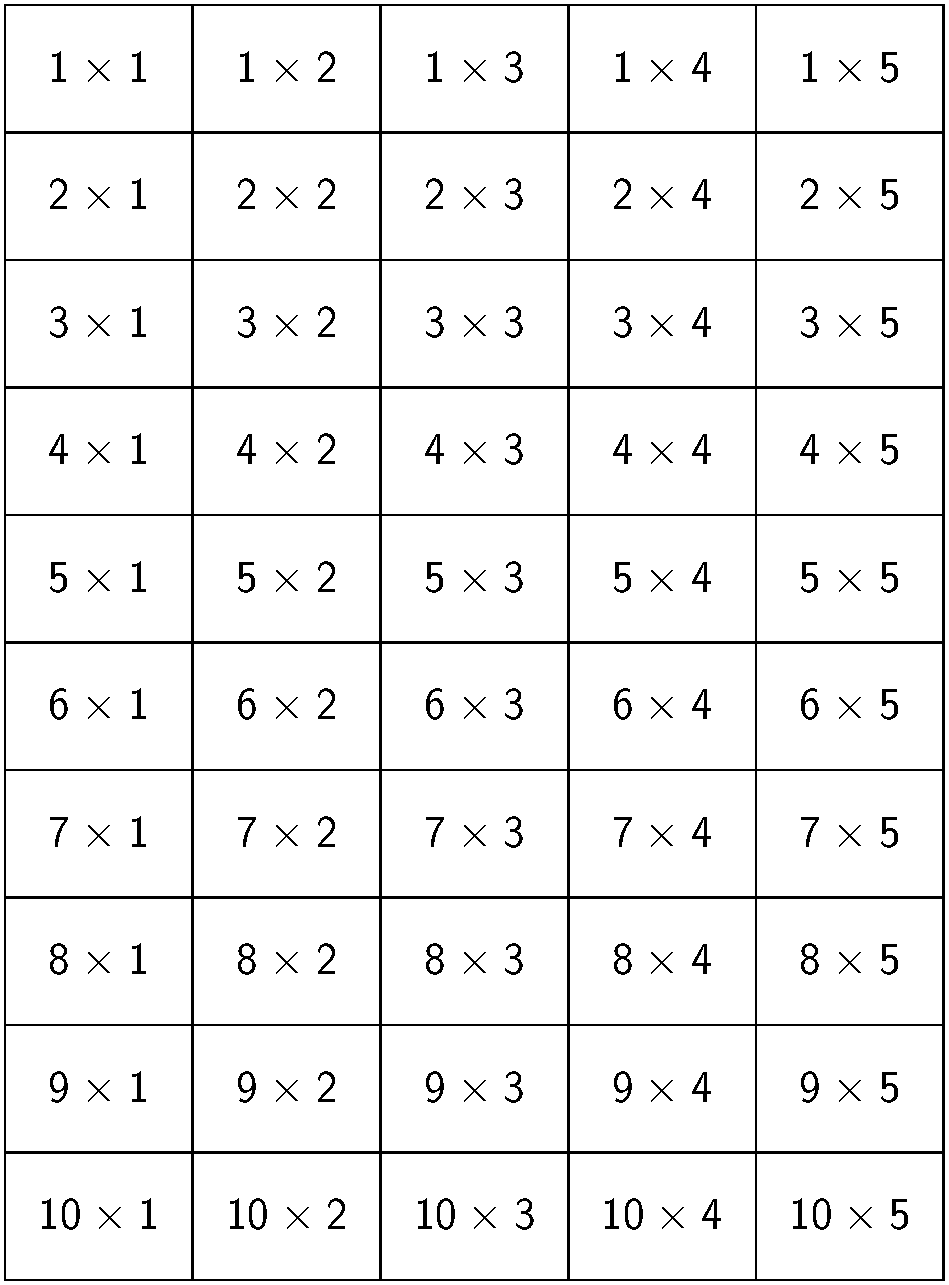
\includegraphics{clasificacionTarjetas-multiplicacion-tarjetas1.pdf}};

  % Add BLM heading
  \node[below right, font=\bf\LARGE] at (topLeft) {Clasificación tarjetas: Multiplicación};
\end{tikzpicture}


% Página 2
\begin{tikzpicture}

  \setPage

  % tarjetas
  \node (tarjetas) at ([yshift=-3ex]center) {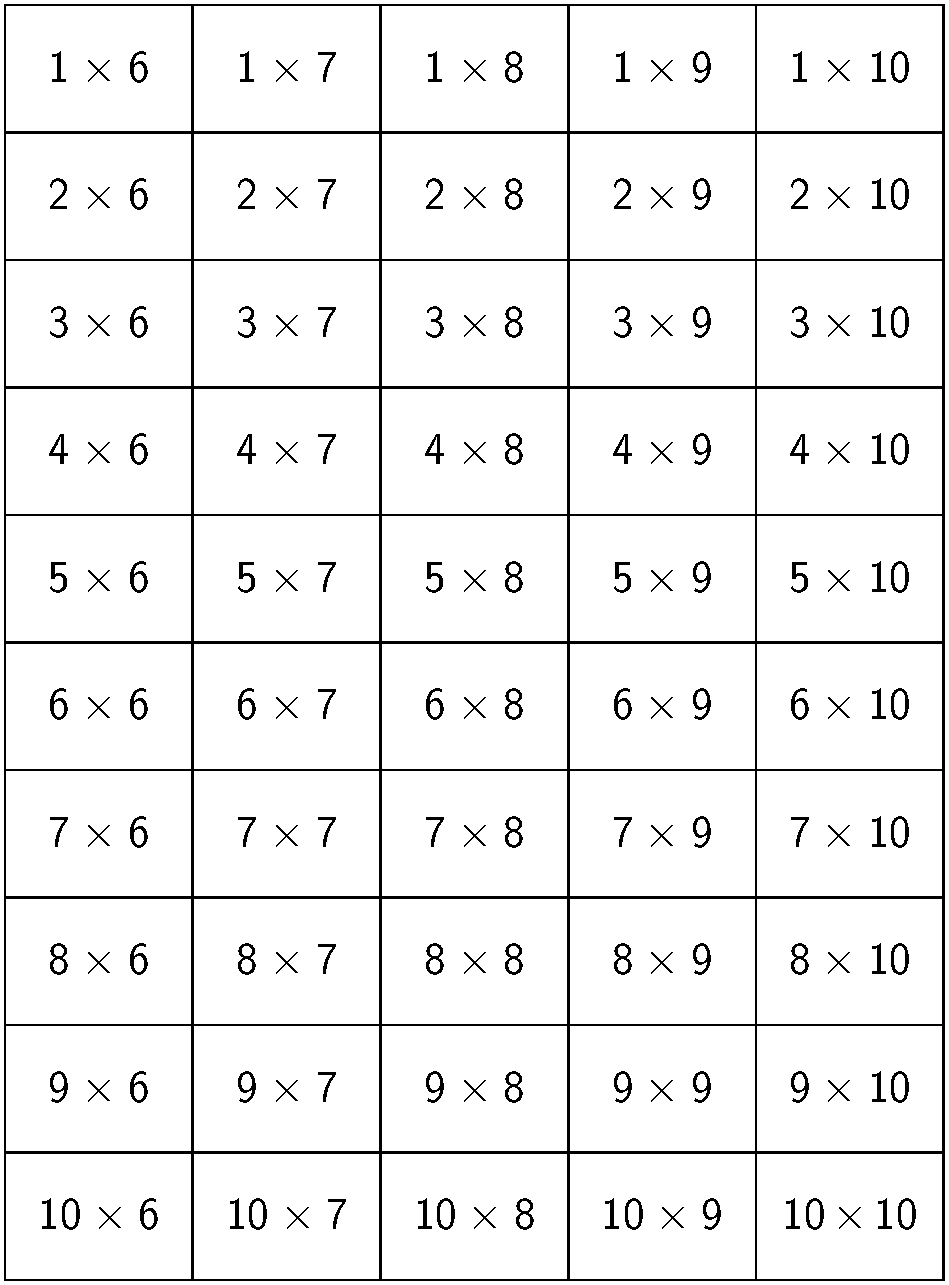
\includegraphics{clasificacionTarjetas-multiplicacion-tarjetas2.pdf}};
\end{tikzpicture}


\end{document}